\begin{center} % Tittelen på dokumentet, sentrert, stor og i bold skrift
\LARGE{\textbf{Eksperiment 1 - Destillasjon og kokepunkt}}
\end{center}
[Alt som står i firkantklammer og fet skrift er instruksjoner/kommentarer som skal fjernes, eller erstattes, unntatt enhetene i datatabeller. Se ellers vedlegg i oppgaveheftet for organisk-lab om oppsett av rapport.]
\section*{Sammendrag}
Formålet med dette eksperimentet var å separere en blanding av sykloheksan og n-butanol, både ved enkel og fraksjonert destillasjon, for å bestemme blandingsforholdet mellom dem. En ukjent prøve ble også identifisert ved bestemmelse av kokepunkt. Blandingsforholdet ble bestemt, ved enkel destillasjon til [FYLL INN HER, f.eks. 1:1], og ved fraksjonert destillasjon til [FYLL INN HER, f.eks. 1:1]. Prøve [FYLL INN HER, f.eks. 2.1] ble identifisert som [FYLL INN HER, f.eks. etanol].




\section{Teori}

\subsection{Kokepunkt for en væske}

De fleste væsker er i en likevekt med sin gassform, og andelen i gassform er avhengig av både temperatur og ytre trykk.\cite{raymond2013general2nd} De molekylene som er i gassform yter det som kalles damptrykk på omgivelsene. Den temperaturen der damptrykket over væskeflaten er lik det eksterne trykket er definert som væskens kokepunkt. 

\subsection{Dalton's lov}

I en blanding av gasser vil hver gass yte et trykk på omgivelsene; Dette kalles for partialtrykket av gassen. Dalton’s lov (se Ligning \ref{eq:dalton}) sier at det totale trykket som gassblandingen yter på omgivelsene er lik summen av de partielle trykkene til komponentene i blandingen.\cite{harwood1999experimental}

\begin{equation}\label{eq:dalton}
    P_{total}= \sum_{i=1}^{n} P_i = P_1 + P_2 + P_3 + ... + P_n 
\end{equation}

\subsection{Raoult's lov}

Raoult’s lov sier at damptrykket til en forbindelse i væskefase, i en ideell blanding med andre væsker, reduseres proporsjonalt med molbrøken til forbindelsen.\cite{harwood1999experimental} Dette er vist i Ligning \ref{eq:Raoult}, der P$_1^*$ er damptrykket over den rene væsken ved samme temperatur, og x$_1$ er molbrøken til væsken.

\begin{equation}\label{eq:Raoult}
    P_1 = P_1^* \times x_1
\end{equation}

\subsection{Kokepunkt for en ideell blanding av væsker}

Ved å kombinere definisjonen for kokepunkt med Dalton og Raoults lover kan det utledes at; For en ideell blanding av væsker vil blandingen koke når summen av partialtrykkene er lik det eksterne trykket. I Ligning \ref{eq:ideell_blanding} er dette vist for en tenkt, ideell blanding av to væsker.

\begin{equation}\label{eq:ideell_blanding}
    P_{total}=P_1 + P_2 = P_1^*\times x_1 + P_2^* \times x_2
\end{equation}

Siden summen av molbrøkene pr. definisjon er 1, kan det videre utledes at det totale trykket må ligge mellom de to «rene» trykkene, se Ligning \ref{eq:ideell_blanding_2}. Dette betyr at kokepunktet til en ideell blanding må ligge mellom kokepunktene til de to rene komponentene. 

\begin{equation}\label{eq:ideell_blanding_2}
    P_{total}=P_1^* \times x_1 + P_2^*  \times (1-x_1 ) = P_2^* - (P_2^* - P_1^* ) \times x_1
\end{equation}

\subsection{Destillasjon}

Destillasjon er en teknikk for å separere flyktige væsker fra andre væsker eller faste stoffer, basert på forskjeller i kokepunkt.\cite{harwood1999experimental} Prinsippet er at den flyktige væsken fordampes til gassform og overføres til en annen beholder, der den kondenseres tilbake til væskeform (destillat). Forskjellen i damptrykk for de rene væskene fører til at dampen over en blanding vil ha en høyere andel av den mest flyktige komponenten, enn væskeblandingen. Når dampen kjøles ned senere vil destillatet derimot ha samme sammensetning som dampen det kondenserte fra. Destillatet vil derfor ha en høyere konsentrasjon av komponenten med lavest kokepunkt, enn den opprinnelige blandingen. 
Det finnes flere metoder for å destillere, noen av de vanligste inkluderer: Enkel destillasjon, fraksjonert destillasjon, destillasjon under redusert trykk, kulerørdestillasjon, mikrodestillasjon, og dampdestillasjon. 

\subsubsection{Enkel destillasjon}

I en enkel destillasjon varmes en væskeblanding opp til sitt kokepunkt, dampen ledes via et destillasjonshode over i en kjøler der den kondenserer, destillatet renner ut og samles i en annen beholder. Oppsettet for en slik destillasjon er vist i Figur \ref{fig:enkel}. 

\begin{figure}[htb!]
    \centering
    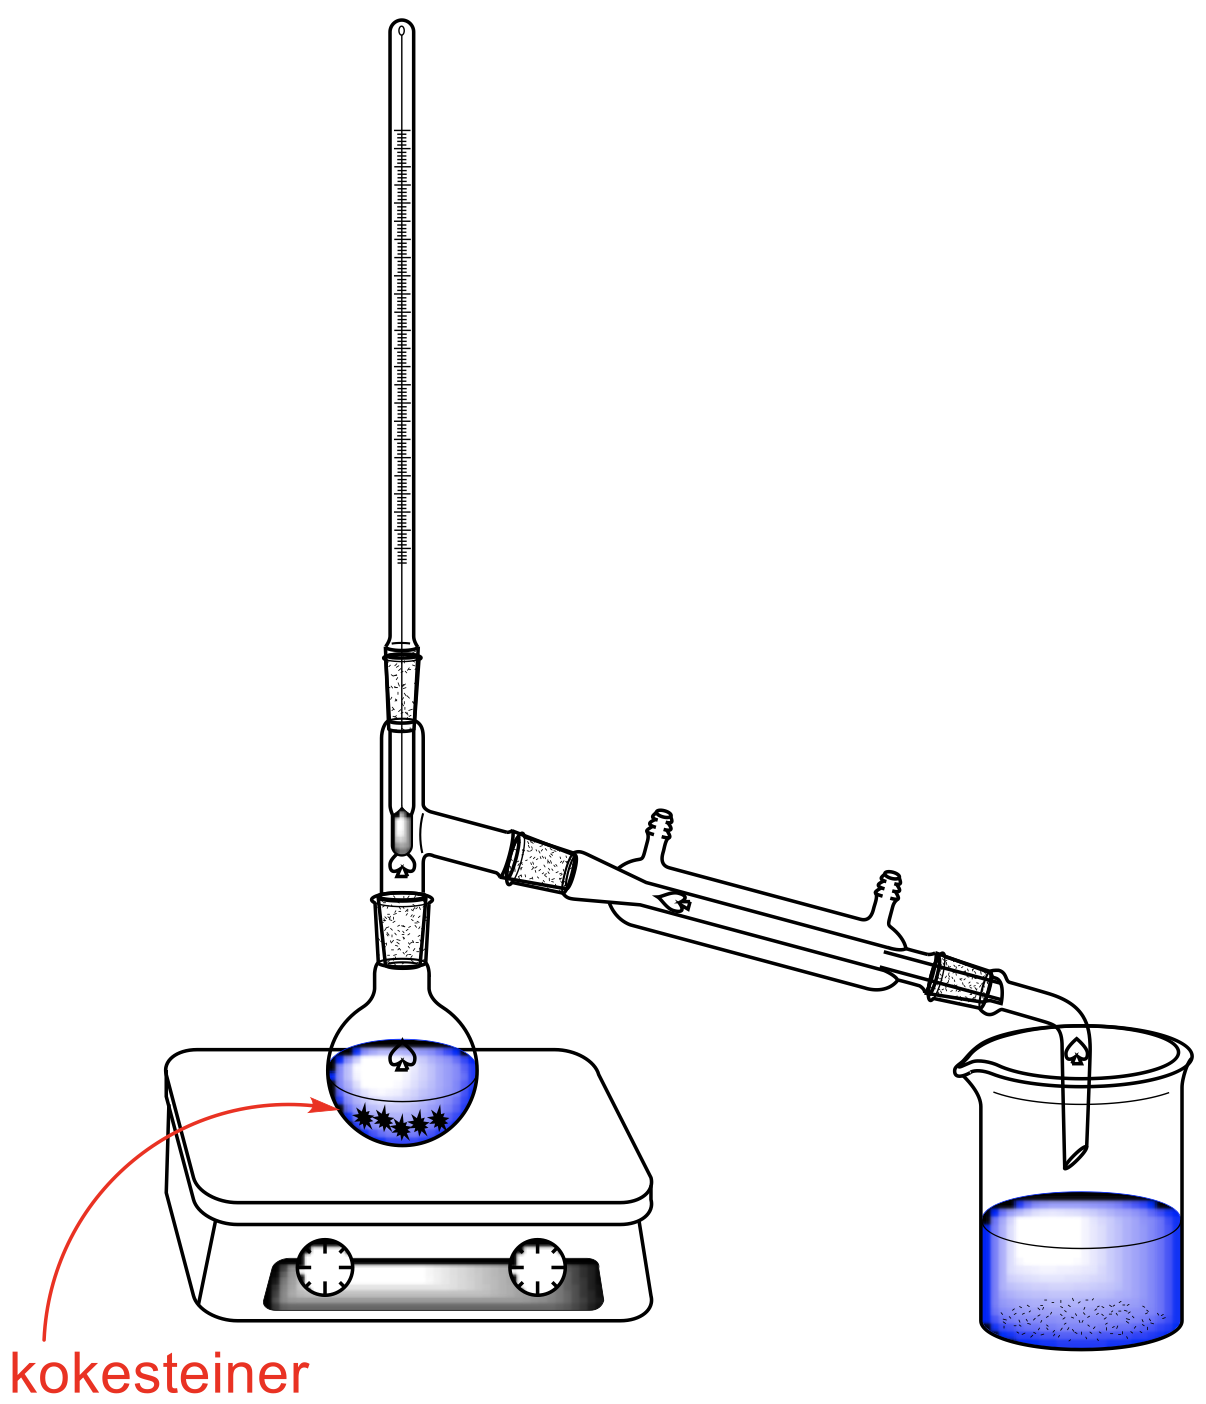
\includegraphics[width=7cm]{Figurer/Enkel_destillasjon.png}
    \caption{Oppsett av utstyr for enkel destillasjon}
    \label{fig:enkel}
\end{figure}

\subsubsection{Fraksjonert destillasjon}

Fraksjonert destillasjon ligner på enkel, men det brukes en fraksjoneringskolonne mellom destillasjonshodet og rundkolben med væskeblandingen. I fraksjoneringskolonnen vil dampen kondensere og fordampe gjentatte ganger på grunn av den store overflaten i kolonnen. I praksis fungerer dette som å gjennomføre mange enkle destillasjoner i serie, med stadig høyere konsentrasjon av den mest flyktige komponenten. Oppsettet for en slik destillasjon er vist i Figur \ref{fig:fraksjonert}.

\begin{figure}[htb!]
    \centering
    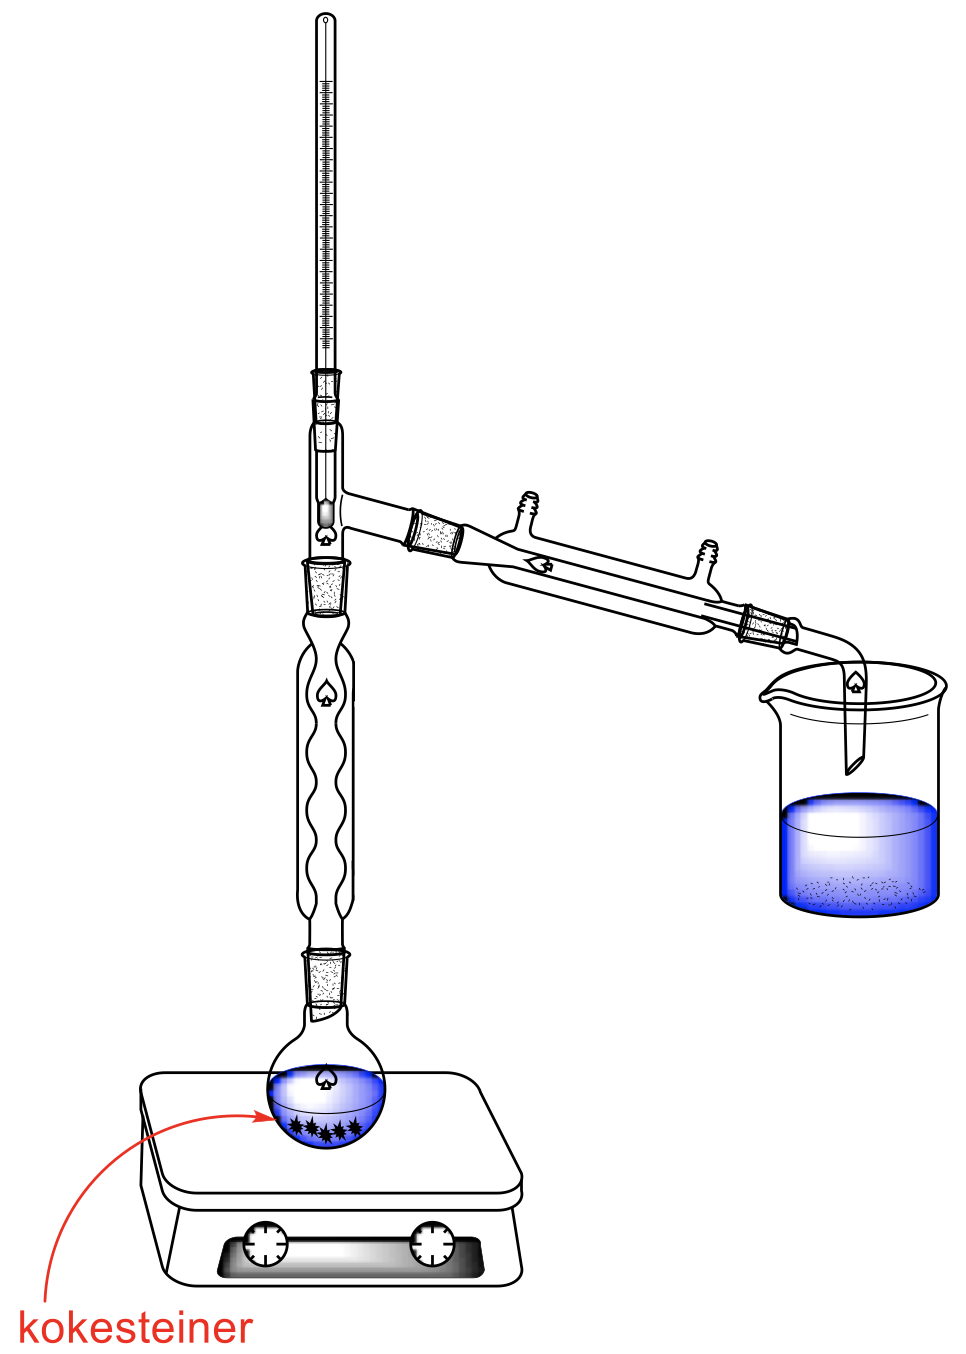
\includegraphics[width=7cm]{Figurer/Fraksjonert_destillasjon.png}
    \caption{Oppsett av utstyr for fraksjonert destillasjon}
    \label{fig:fraksjonert}
\end{figure}


\section{Fysikalske data}
Relevante fysikalske data til forbindelser brukt i dette forsøket er vist i Tabell \ref{tab:fys_data}.
\begin{table}[ht!]
	\begin{center}
		\caption{Fysikalske data for aktuelle forbindelser \cite{CRC}}
		\label{tab:fysdata}
		\begin{tabular}{l c c}
		\toprule
		Forbindelse & Kokepunkt[\si{\celsius}]\\
		\midrule
		\textit{n}-Propylamin & 47\\
		Aceton & 56\\
		Metanol & 65 \\
		Etylacetat & 77 \\
		2-Propanol & 82 \\
		Butanon & 80 \\
		1-Propanol & 97 \\
		Sykloheksan & 81 \\
		Vann & 100 \\
		\textit{n}-Butanol & 117 \\
		\bottomrule
		\end{tabular}
	\end{center}
\end{table}



\section{Eksperimentelt}

\subsection{Bestemmelse av kokepunkt}\label{sec:eksperimentelt_1}

Et gradert reagensrør ble festet til et termometer med strikk og et kapillærrør ble lagt ned i reagensrøret med den åpne enden ned. Reagensrør og termometer ble montert i et oljebad som på en varmeplate. En ukjent væske (ca. 1 mL) ble overført til reagensrøret og oppvarmet til gassbobler begynte å strømme raskt ut av kapillærrøret. På dette tidspunktet ble oppvarmingen slått av og varmeplaten ble byttet med en labjekk. Temperaturen sank gradvis og færre gassbobler kom ut av kapillærrøret.  Temperaturen da siste gassboble gikk ut og væske gikk inn i kapillærrøret ble registrert. Denne temperaturen ble rapportert som kokepunktet til den ukjente væsken. 

\subsection{Destillasjon}

Det ble gjennomført to forskjellige destillasjoner, enkel og fraksjonert. Noen kokesteiner og en blanding av sykloheksan og n-butanol (60 mL) ble overført til en rundkolbe, og resten av oppsettet ble montert som vist i Figur \ref{fig:enkel} og Figur \ref{fig:fraksjonert} (for hhv. enkel og fraksjonert destillasjon). Det ble gradvis varmet opp i en varmekappe til dråpehastigheten av destillat var 20-30 dråper/min. Temperaturen i destillasjonshodet ble avlest ved første dråpe destillat, og deretter for hver andre mL (2, 4, 6 osv.). Ved 55 mL oppsamlet destillat ble varmen skrudd av og destillasjonen stoppet for å unngå tørrkoking.

\section{Resultater}

\subsection{Bestemmelse av kokepunkt}

Kokepunktet for den ukjente prøven ble bestemt i henhold til prosedyren i avsnitt \ref{sec:eksperimentelt_1}. 

\subsection{Destillasjonsgraf}


\section{Diskusjon}
